\documentclass{beamer}
\usepackage[utf8]{inputenc}
\usepackage{polski}
\usepackage{graphicx}
\usepackage{float}
\usepackage{indentfirst}
\usepackage{multicol}

\usetheme{Warsaw}

% items enclosed in square brackets are optional; explanation below
\title[Roboty mobilne poruszające się z poślizgami]{Algorytmy sterowania robotów mobilnych poruszających się z poślizgami}
\author[Paweł Bogner]{Paweł Bogner\\ \vspace{5pt}\footnotesize Promotor: Prof. Krzysztof Tchoń\\ }
\institute[]{
  Politechnika Wrocławska\\
  Wydział Elektroniki\\
  Automatyka i Robotyka\\
  Robotyka
}
\date{}
\newcommand{\ud}{\mathrm{d}}
\newcommand{\rot}{\mathrm{Rot}}
\newcommand{\tr}{\mathrm{Trans}}
\begin{document}

\begin{frame}[plain]
  \titlepage
\end{frame}

\begin{frame}
  \frametitle{Plan prezentacji}
  \tableofcontents
\end{frame}

\section{Wprowadzenie}
\begin{frame}{Cele pracy}
\begin{itemize}
\item Badanie modeli robotów mobilnych poruszających się z poślizgami,
\item planowanie ruchu dla tych obiektów metodą endogenicznej przestrzeni konfiguracyjnej,
\item sprawdzenie działania tej metody planowania dla obiektów z nieciągłym modelem tarcia.
\end{itemize}
\end{frame}

\section{Badane obiekty}
\subsection{Monocykl}
\begin{frame}{Monocykl}
\begin{center}
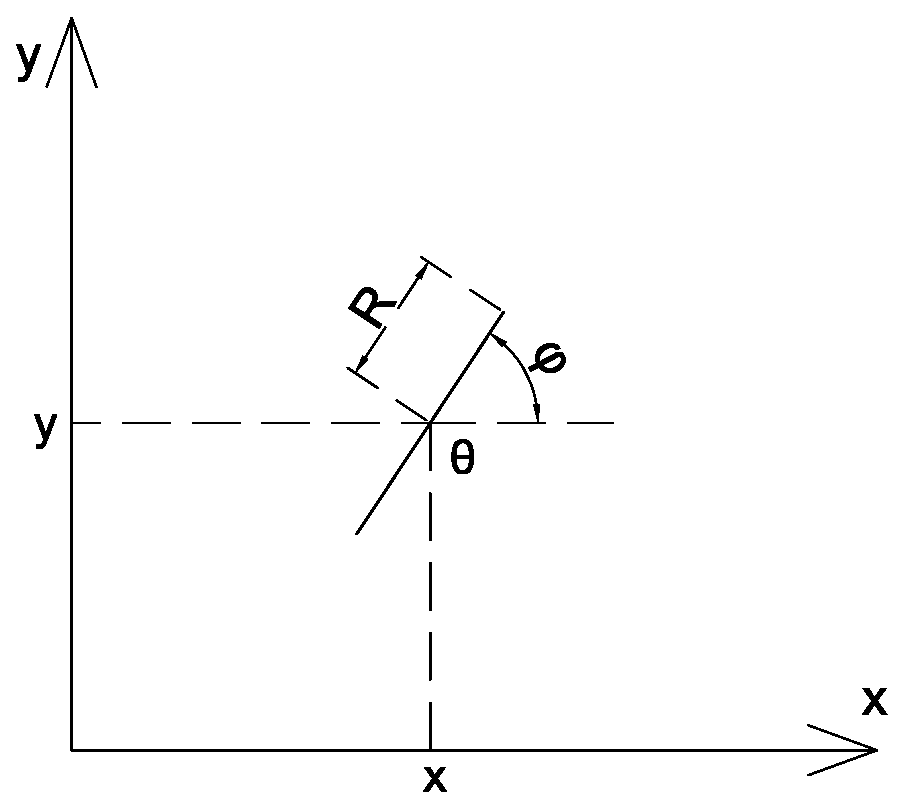
\includegraphics[width=0.6\textwidth]{img/uni.eps}
\end{center}
\end{frame}

\subsection{Manipulator mobilny RobRex}
\begin{frame}{Platforma mobilna Rex}
\begin{center}
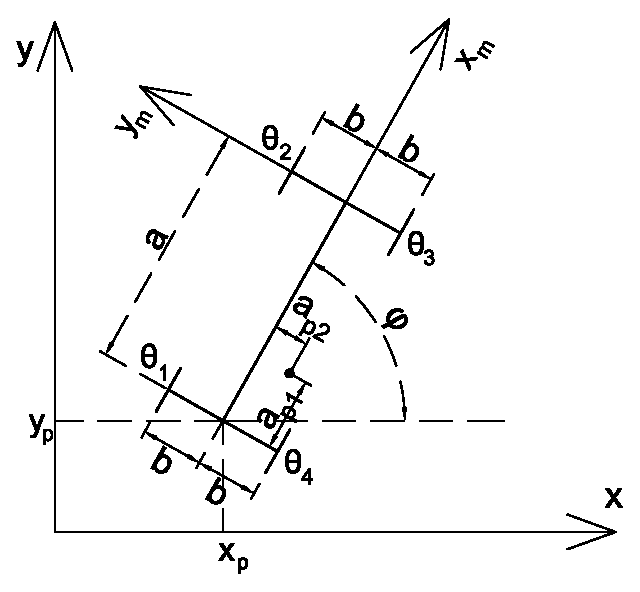
\includegraphics[width=0.6\textwidth]{img/robrex.eps}
\end{center}
\end{frame}

\begin{frame}{Manipulator}
\begin{center}
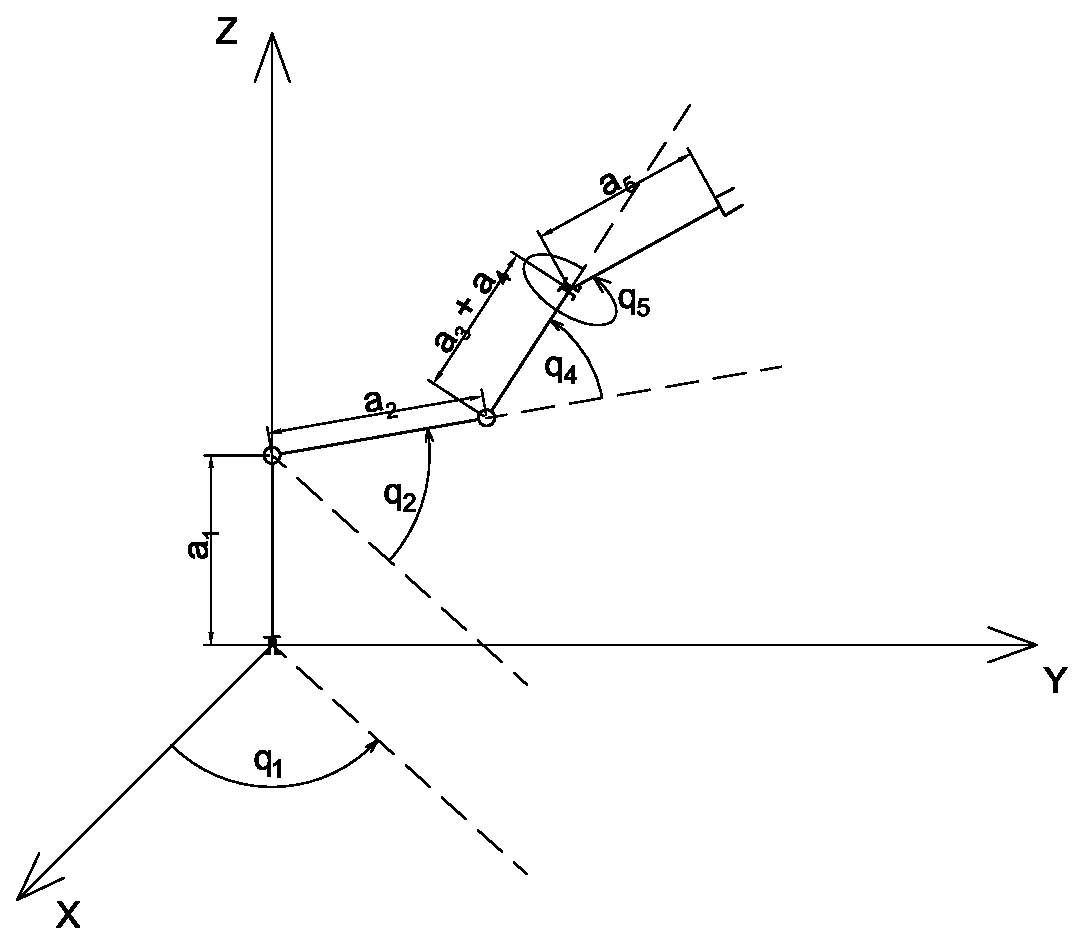
\includegraphics[width=0.6\textwidth]{img/manip.eps}
\end{center}
\end{frame}

\subsection{Model tarcia}
\begin{frame}{Nieciągły model tarcia}
\begin{center}
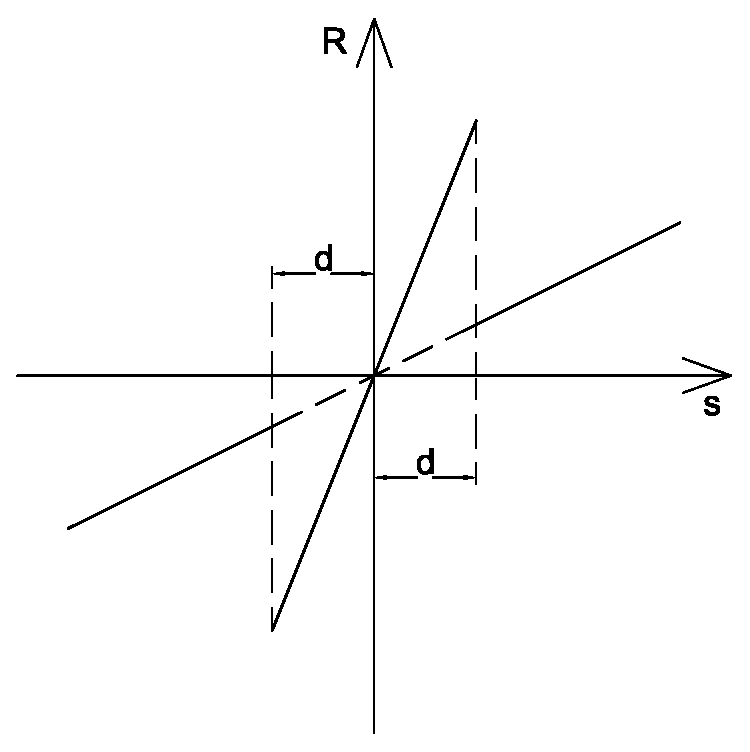
\includegraphics[width=0.6\textwidth]{img/discont.eps}
\end{center}
\end{frame}

\section{Przykładowe wyniki}
\subsection{Platforma mobilna Rex --- ciągły model tarcia}
\begin{frame}{Ścieżka}
\begin{center}
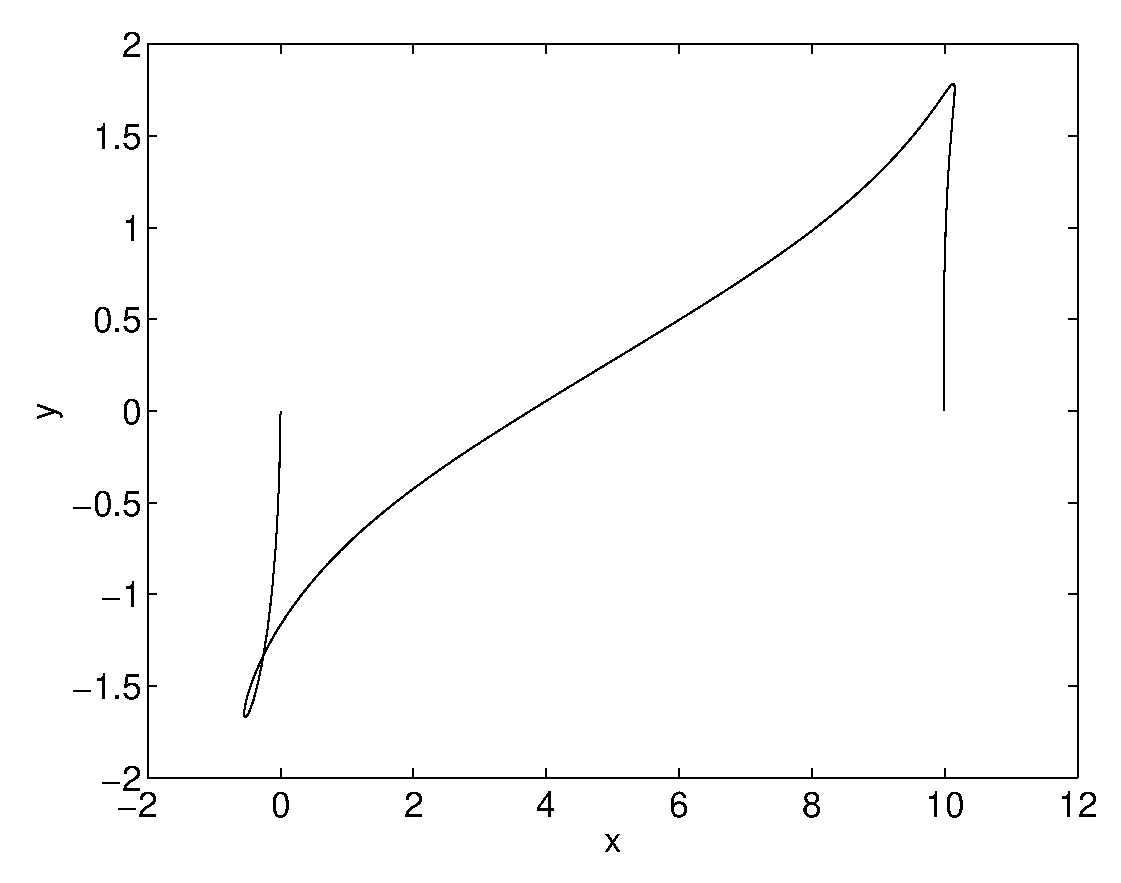
\includegraphics[width=0.6\textwidth]{img/final_15_1_20_path.eps}
\end{center}
\end{frame}
\begin{frame}{Poślizgi}
\begin{center}
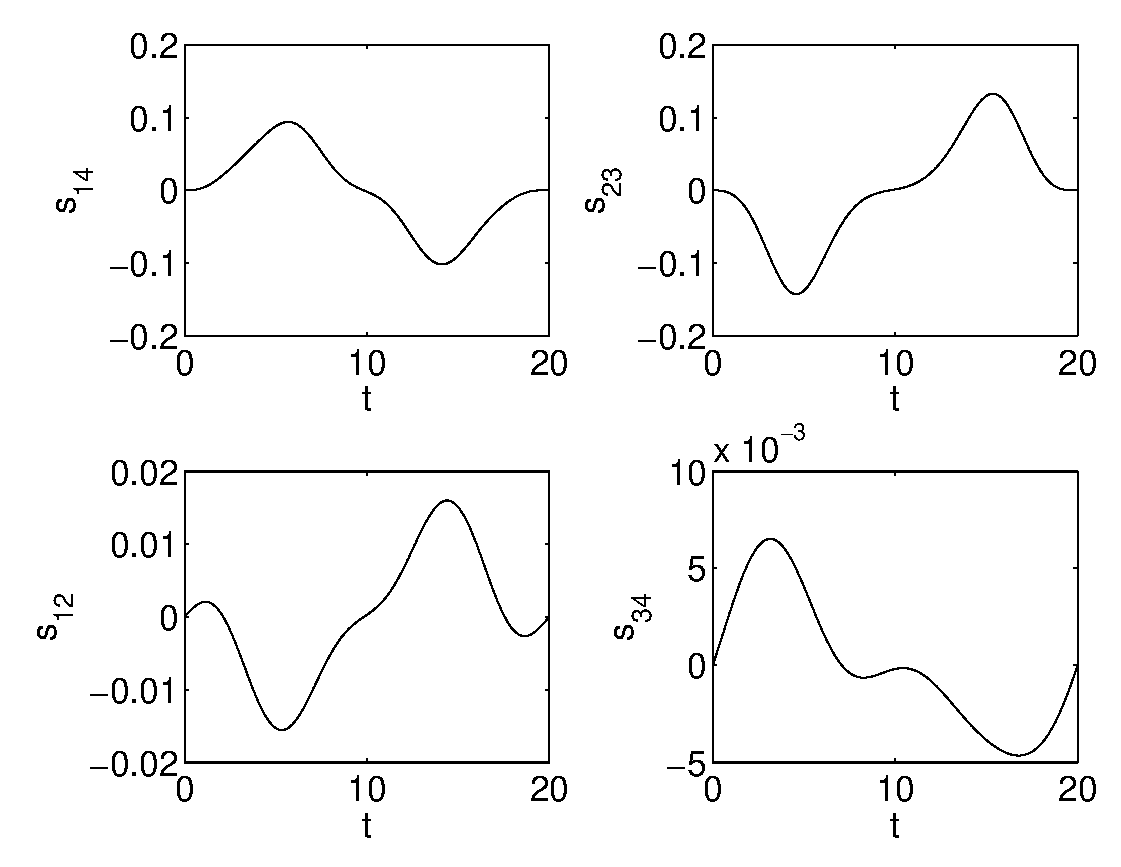
\includegraphics[width=0.6\textwidth]{img/final_15_1_20_slips.eps}
\end{center}
\end{frame}
\begin{frame}{Sterowania}
\begin{center}
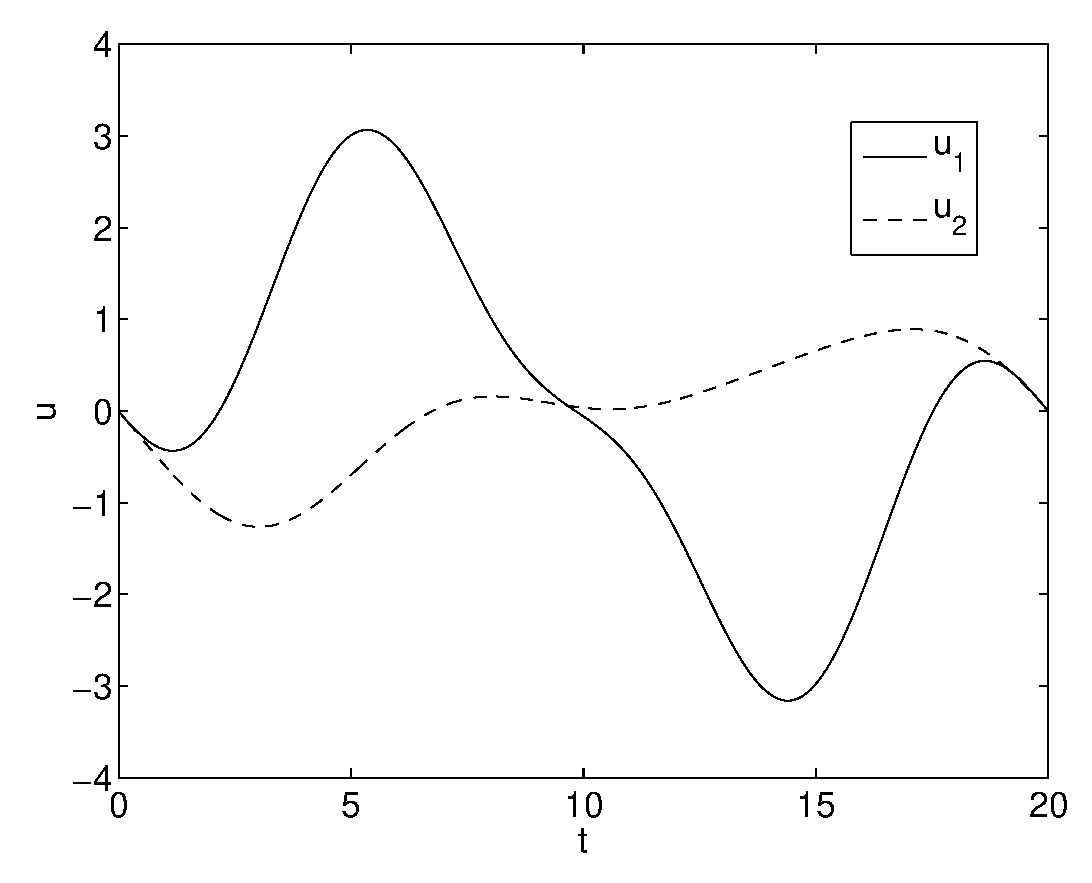
\includegraphics[width=0.6\textwidth]{img/final_15_1_20_u.eps}
\end{center}
\end{frame}
\subsection{Monocykl --- nieciągły model tarcia}
\begin{frame}{Ścieżka}
\begin{center}
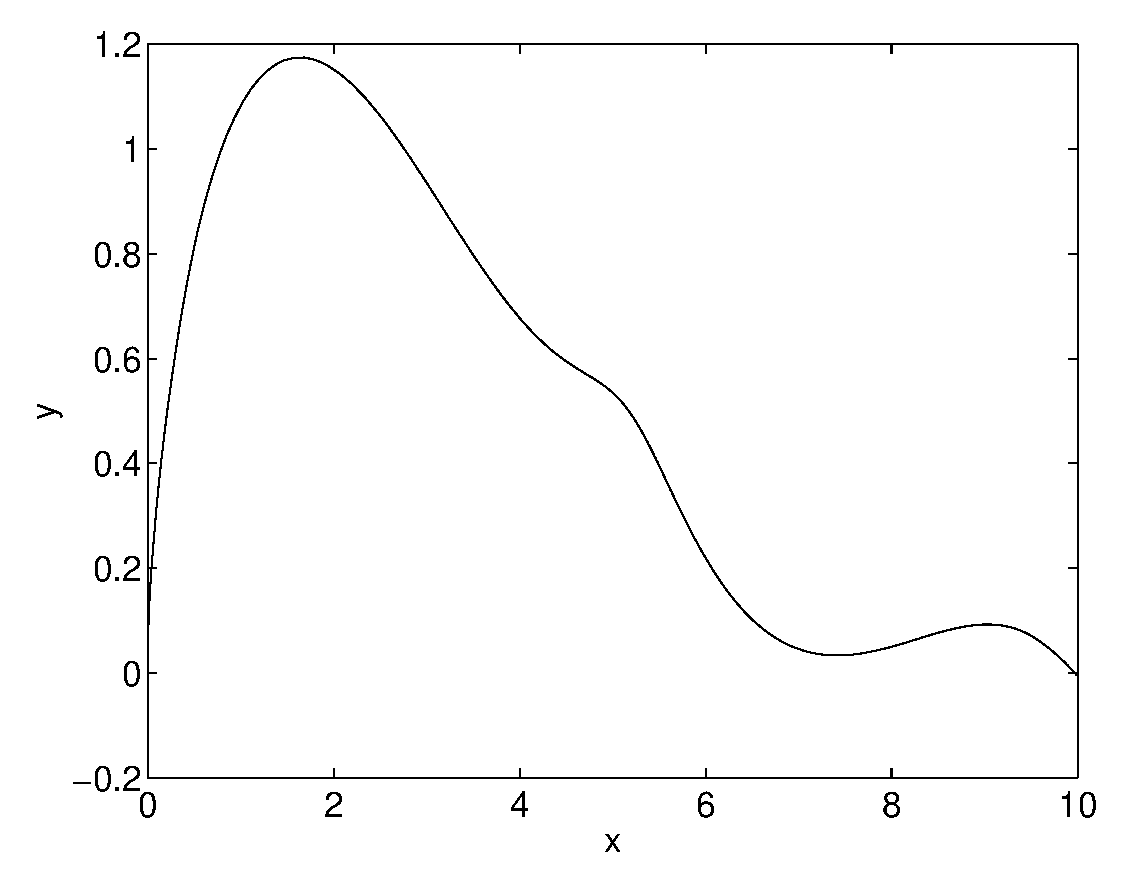
\includegraphics[width=0.6\textwidth]{img/unicycle_path.eps}
\end{center}
\end{frame}
\begin{frame}{Poślizgi}
\begin{center}
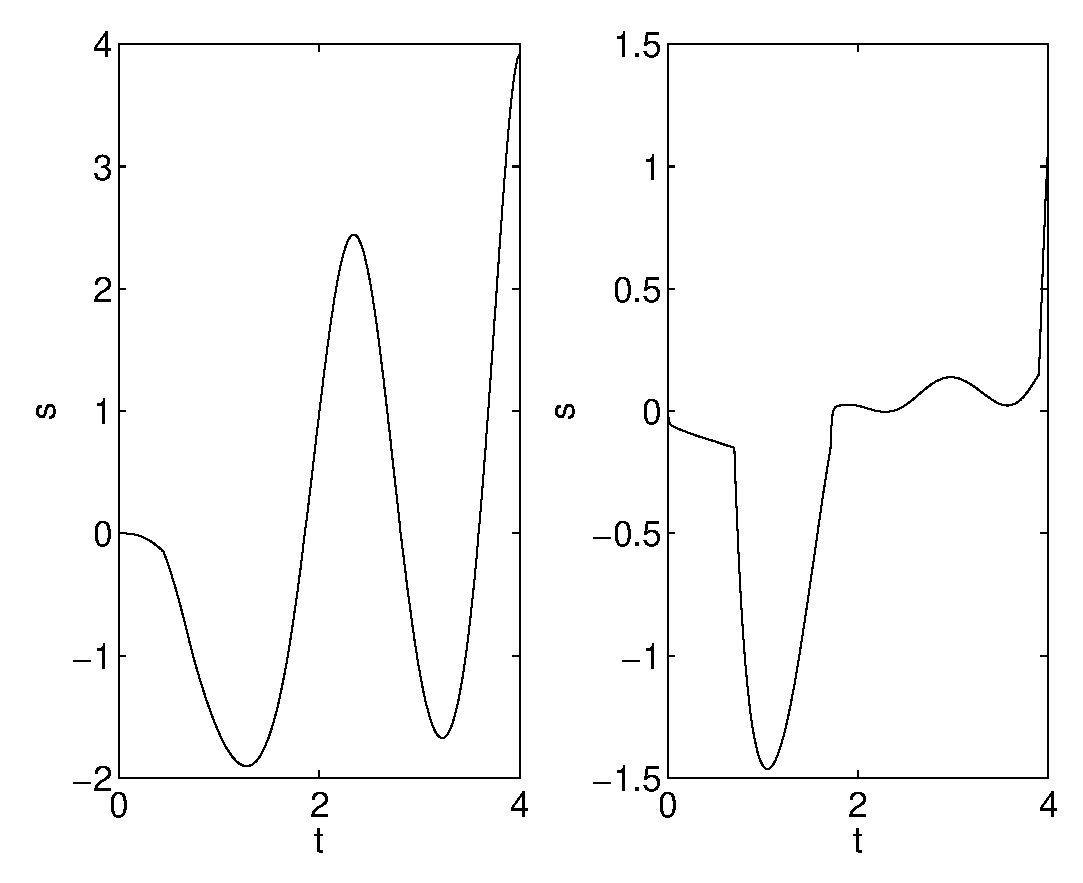
\includegraphics[width=0.6\textwidth]{img/unicycle_slips.eps}
\end{center}
\end{frame}
\begin{frame}{Sterowania}
\begin{center}
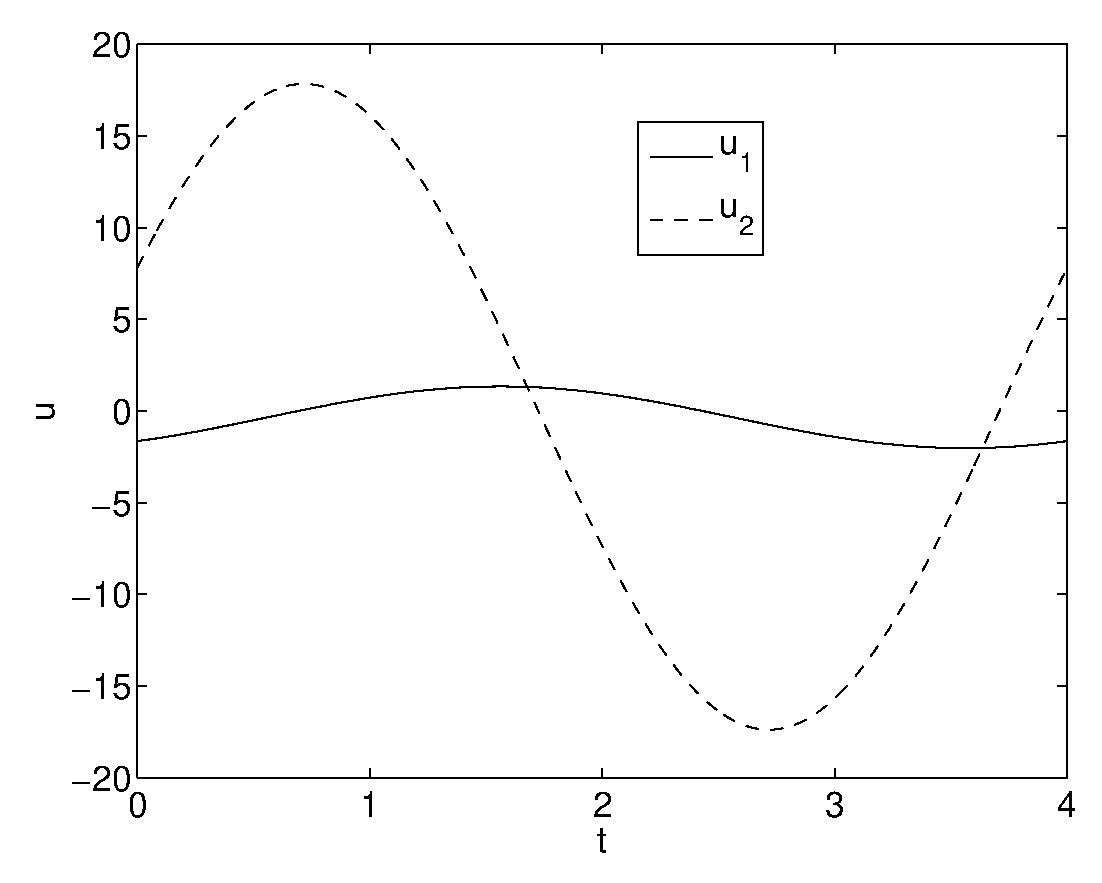
\includegraphics[width=0.6\textwidth]{img/unicycle_u.eps}
\end{center}
\end{frame}
\subsection{Platforma mobilna Rex --- nieciągły model tarcia}
\begin{frame}{Ścieżka}
\begin{center}
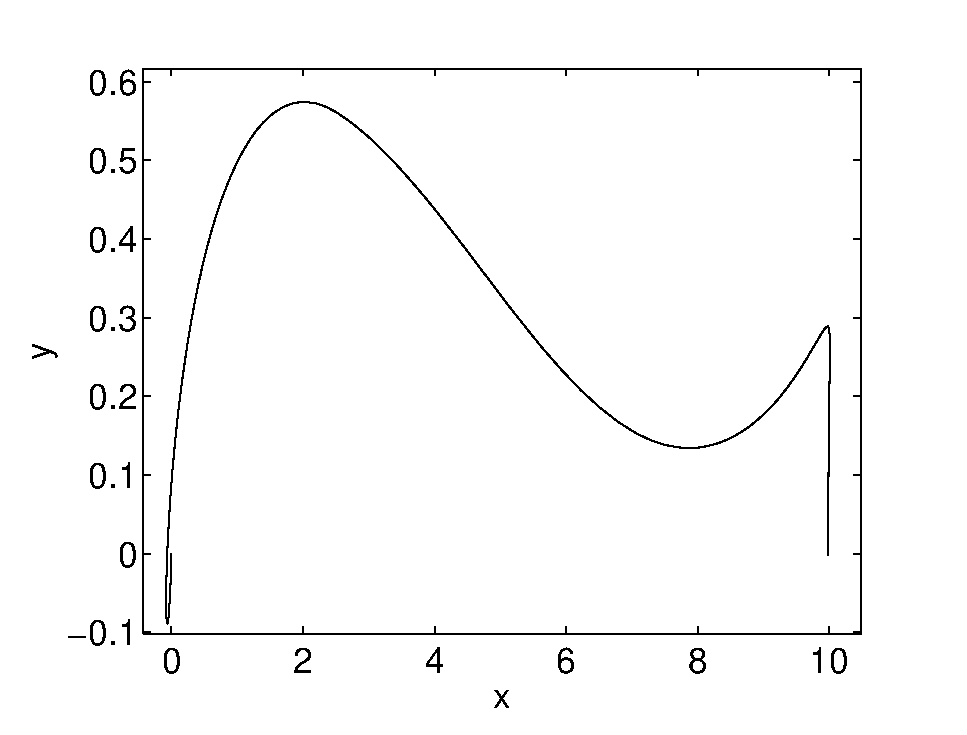
\includegraphics[width=0.6\textwidth]{img/discont_ok_path.eps}
\end{center}
\end{frame}
\begin{frame}{Poślizgi}
\begin{center}
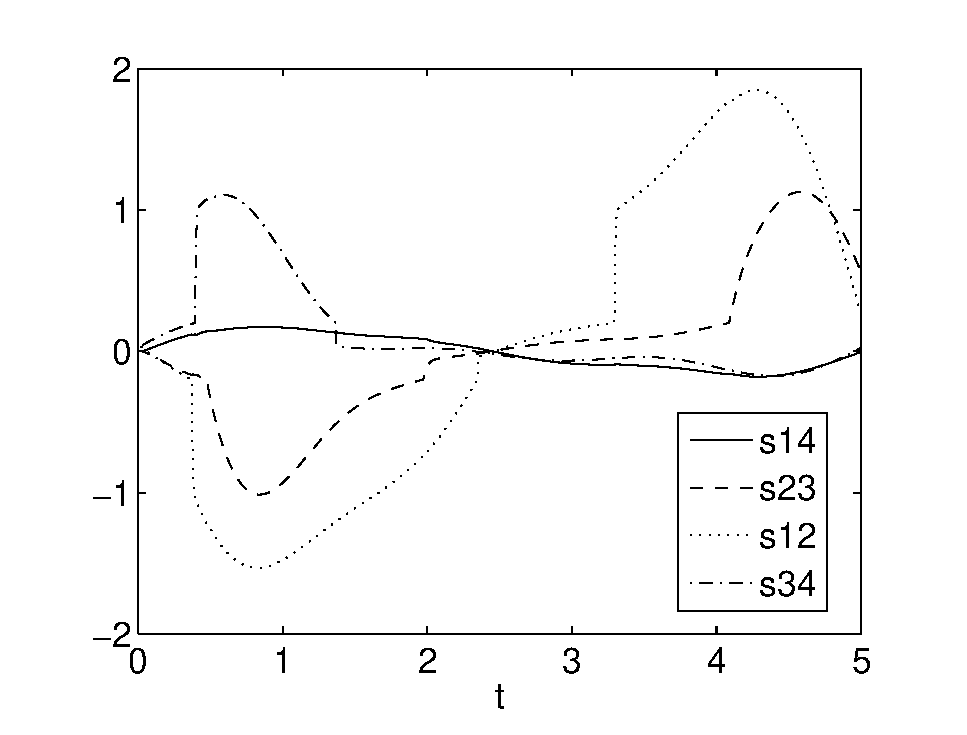
\includegraphics[width=0.6\textwidth]{img/discont_ok_slips.eps}
\end{center}
\end{frame}
\begin{frame}{Sterowania}
\begin{center}
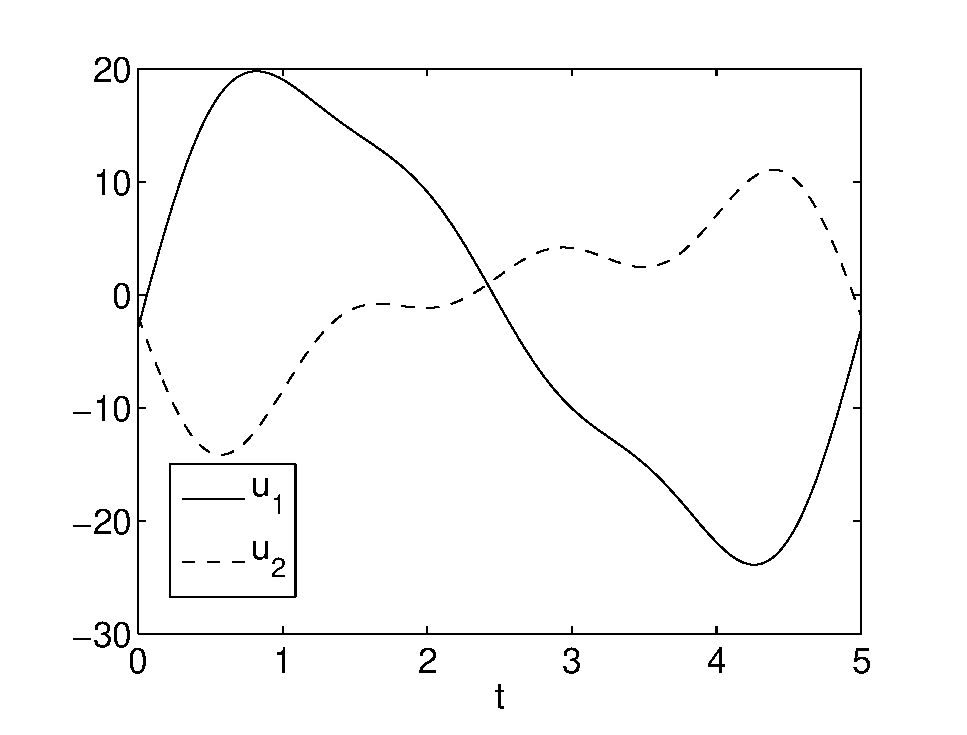
\includegraphics[width=0.6\textwidth]{img/discont_ok_u.eps}
\end{center}
\end{frame}
\section{Podsumowanie}
\begin{frame}{Wnioski}
\begin{itemize}
\item Skracanie horyzontu czasowego sterowania zwiększa wartości sterowań.
\item Wysoki współczynnik tarcia powoduje zanikanie poślizgów.
\item Wysoki współczynnik tarcia poprzecznego utrudnia skręcanie platformy, może to powodować osobliwości.
\item Metoda endogenicznej przestrzeni konfiguracyjnej daje dobre rezultaty dla planowania ruchu robotów poruszających się z poślizgami z uwzględnieniem ich dynamiki.
\item Metoda ta w ogólności nie jest zbieżna dla modeli zawierających nieciągłości.
\item Zbieżność algorytmu można uzyskać jedynie w szczególnych przypadkach.
\end{itemize}
\end{frame}

\end{document}
